\section*{Attachment 2: Formative project for practicum exam}

\subsection*{General (important) information}
\begin{itemize}
\item The assignment must be implemented using C\# or F\#.
\item The only library tools you are allowed to use are: arrays, lists, and math functions. Other data structures or functions on data structures covered by the course must be implemented \textbf{by hand}.
\end{itemize}

\subsection*{Introduction to the framework}
The exercises will be based on the simulation of a city, containing houses and special buildings (represented through ancient civilization temples), all connected by streets. The student must implement algorithms to answer some queries on the simulated city.
To set up the framework, follow these instructions:

\begin{itemize}
\item Download and install the latest version of Visual Studio Community (\url{https://www.visualstudio.com/en-us/downloads/download-visual-studio-vs.aspx}); choose ``F\# language" during \textit{custom setup}; 
\item Download the project framework from N@tschool (or Github) and open the .sln file; if it is not already set, right click on \texttt{EntryPoint} project (in the solution explorer) and select ``Set as startup project";
\item The functions you have to program are contained in the file \texttt{Program.cs}; for now there are stub versions of the function implementations that you have to replace with yours;
\item Compile the project in debug mode and run it with Ctrl+F5;
\item A window opens asking you which assignment you want to execute: choose a number between 1 and 4 \footnote{In the application, assignment 3 corresponds to exercise 3.1; assignment 4 corresponds to exercise 3.2.} (or q if you want to close it) and press Ok;
\item The simulation will start. You can move the visual with WASD and zoom with Z (zoom in) and X (zoom out).
\item Exit with ESC. 
\end{itemize}

\newpage
\subsection*{Exercise 1 - Sorting}

\subsubsection*{Goal}
Sort all special buildings by Euclidean distance from a specified house. The Euclidean distance formula is:
\begin{align*}
d(house,building) = \sqrt{(x_{house} - x_{building})^{2} + (y_{house} - y_{building})^{2} } 
\end{align*}
This means that the connection through roads is not relevant in this exercise (everyone has his private helicopter to move around the city).

\subsubsection*{Function signature} 
\begin{lstlisting}
private static IEnumerable<Vector2> SortSpecialBuildingsByDistance(Vector2 house, IEnumerable<Vector2> specialBuildings)
\end{lstlisting}

This function takes as input a house position (\texttt{Vector2 house}) and a list of building positions (\\ \texttt{IEnumerable<Vector2> specialBuildings}) and returns a sorted list of building positions according to their distance from the house position (\texttt{IEnumerable<Vector2>}). Use the \textbf{merge sort} as sorting algorithm. Any implementation not using this technique will not be accepted and evaluated.\\

\subsubsection*{Result}
As you can see from Figure \ref{img:Ex1}, the selected house is highlighted and there is a number above each special building indicating its position in the sorted list of buildings. 

\begin{figure}[!h]
\centering
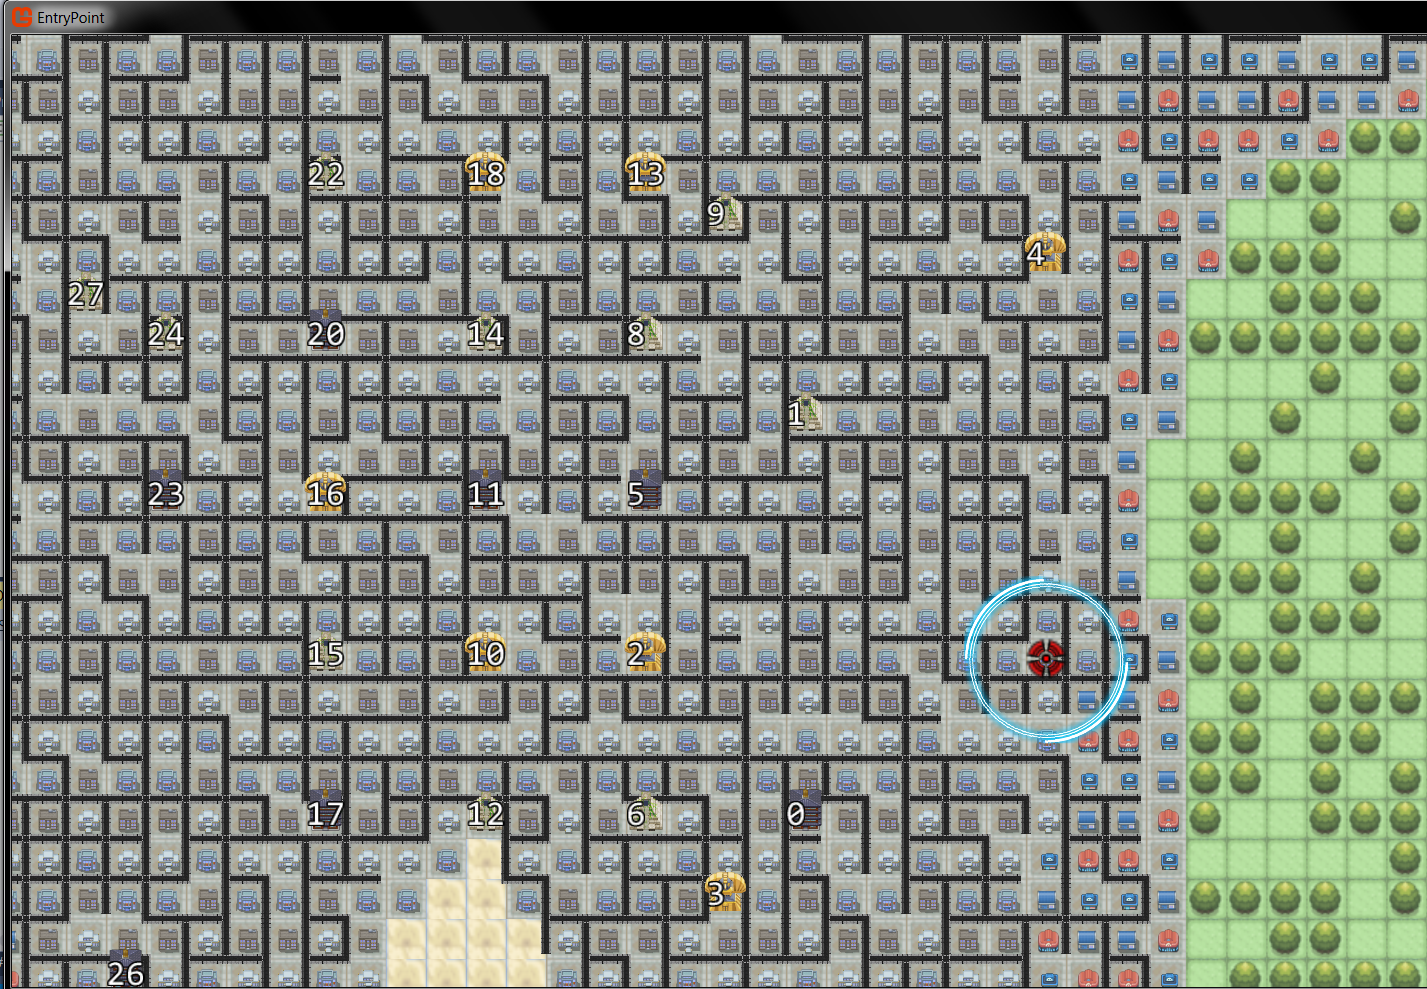
\includegraphics[scale=0.25]{img/exercise1}
\caption{Exercise 1 result}
\label{img:Ex1}
\end{figure}

\newpage
\subsection*{Exercise 2 - Trees}

\subsubsection*{Goal}
Find all the special buildings within a specified distance from each house. Create a \textbf{k-d tree} to organize the special buildings positions in advance (like explained in class). Then look up the tree for each of the requested houses (with the associated distance).

\subsubsection*{Function signature} 
\begin{lstlisting}
private static IEnumerable<IEnumerable<Vector2>> FindSpecialBuildingsWithinDistanceFromHouse(IEnumerable<Vector2> specialBuildings, IEnumerable<Tuple<Vector2, float>> houseAndDistances)
\end{lstlisting}

\noindent
This function takes as input a list of special building positions (\texttt{IEnumerable<Vector2> specialBuildings}), a list of pairs made of a house position and the maximum distance for a special building to be selected (\texttt{IEnumerable<Tuple<Vector2, float>> houseAndDistances}), and returns a list of lists of positions (\\ \texttt{IEnumerable<IEnumerable<Vector2>>}) of selected special buildings (one list for each house).\\

\subsubsection*{Result}
As you can see from Figure \ref{img:Ex2}, each selected house is surrounded by a circle that should contain all the special buildings within the distance associated to such house. The buildings you return are highlighted in blue, the houses in red.

\begin{figure}[!h]
\centering
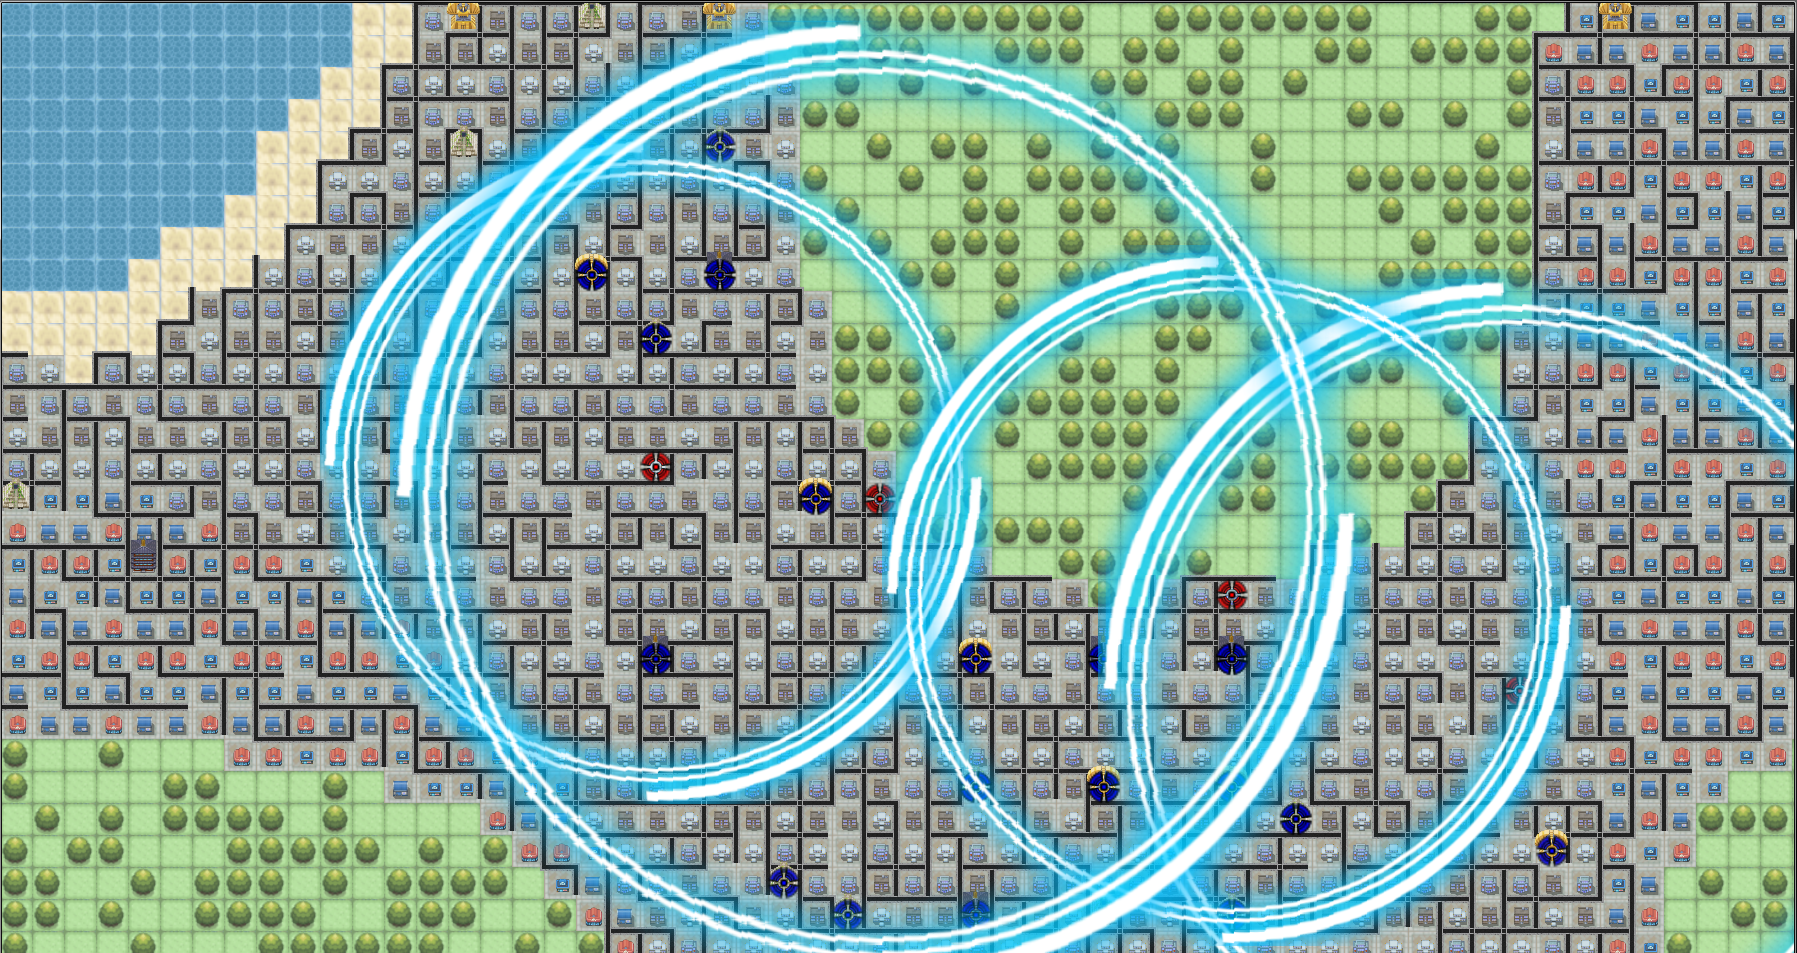
\includegraphics[scale=0.25]{img/exercise2}
\caption{Exercise 2 result}
\label{img:Ex2}
\end{figure}

\newpage
\subsection*{Exercise 3 - Graphs}

\subsubsection*{Goal}
Find the shortest path(s) from a specified house to other special building(s). The shortest path is made of the road sections to use in order to drive from the house to the special building.\\
\textbf{Remark}: This assignment can be solved in two ways, that is using Dijkstra or Floyd Warshall.\\
\textbf{Hint:} In both assignments, you have to build the adjacency matrix using the starting point and endpoint of the road sections. The weight of the edge is the distance between the two points.

\subsection*{Option 1: Dijkstra}
In this assignment we want to compute the minimum path between one house and one special building. 

\subsubsection*{Function signature} 
\begin{lstlisting}
private static IEnumerable<Tuple<Vector2, Vector2>> FindRoute(Vector2 startingBuilding, Vector2 destinationBuilding, IEnumerable<Tuple<Vector2, Vector2>> roads)
\end{lstlisting}

\noindent
This function takes as input the position of the house to start from (\texttt{Vector2 startingBuilding}), the position of the destination (\texttt{Vector2 destinationBuilding}), and a list of road sections, each represented as a pair of starting point and endpoint (\texttt{IEnumerable<Tuple<Vector2, Vector2>> roads}), and returns a list of road sections (\texttt{IEnumerable<Tuple<Vector2, Vector2>>}) forming the shortest path between the house and the destination.\\

\subsubsection*{Result} 
As you can see from Figure \ref{img:Ex3-1}, the house is surrounded by a circle and highlighted in red. The path to the destination is highlighted with coloured dots.

\begin{figure}[!h]
\centering
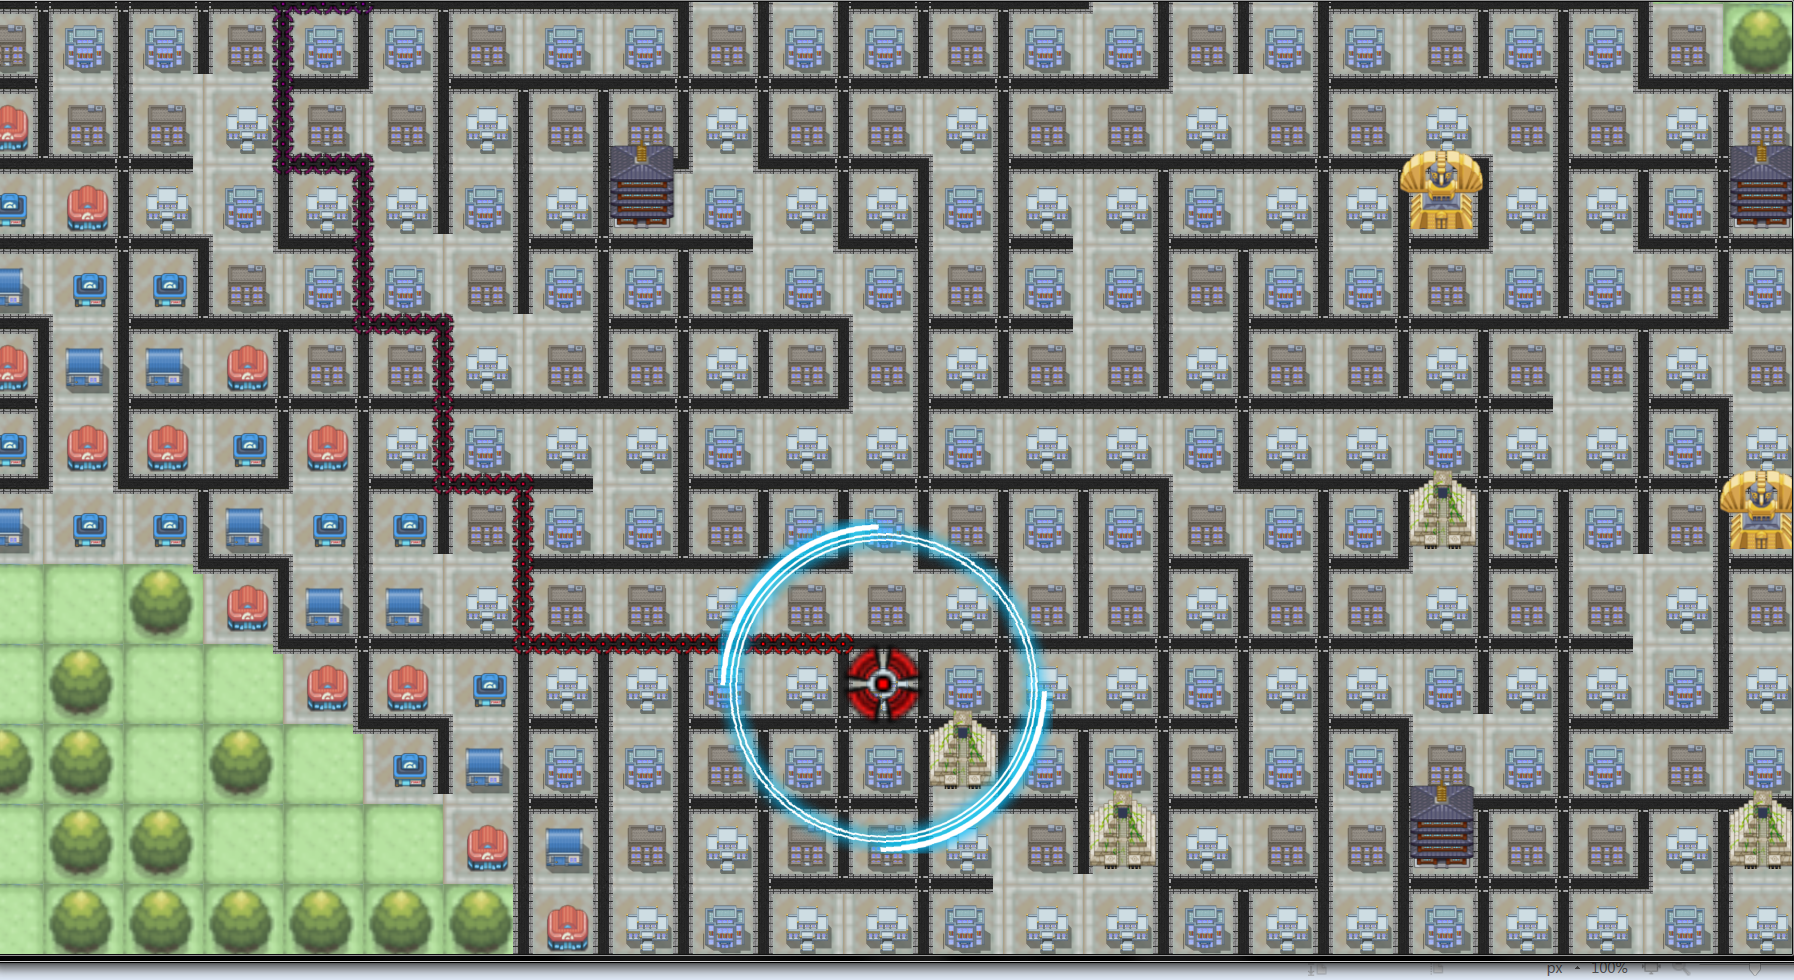
\includegraphics[scale=0.2]{img/exercise3}
\caption{Exercise 3.1 result}
\label{img:Ex3-1}
\end{figure}


\subsection*{Option 2: Floyd Warshall}
In this assignment we want to compute the minimum paths between one house and a list of special buildings. 

\subsection*{Function signature} 
\begin{lstlisting}
private static IEnumerable<IEnumerable<Tuple<Vector2, Vector2>>> FindRoutesToAll(Vector2 startingBuilding, IEnumerable<Vector2> destinationBuildings, IEnumerable<Tuple<Vector2, Vector2>> roads)
\end{lstlisting}

\noindent
This function takes as input the position of the house to start from (\texttt{Vector2 startingBuilding}), the positions of all the destinations (\texttt{IEnumerable<Vector2> destinationBuildings}), and a list of road sections, each represented as a pair of starting point and endpoint (\texttt{IEnumerable<Tuple<Vector2, Vector2>> roads}), and returns a list of shortest paths (\texttt{IEnumerable<IEnumerable<Tuple<Vector2, Vector2>>>}). Each shortest path is referred to one specific destination and is made of a list of road sections.
The function must precompute the all-pairs shortest path with Floyd Warshall algorithm and then extract only the paths requested by the function from the distance and predecessor matrices.\\

\subsection*{Result}
As you can see from Figure \ref{img:Ex3-2}, the house is surrounded by a circle and highlighted in red. The destinations are highlighted in blue. The paths from the house to all destinations are highlighted with coloured dots.

\begin{figure}
\centering
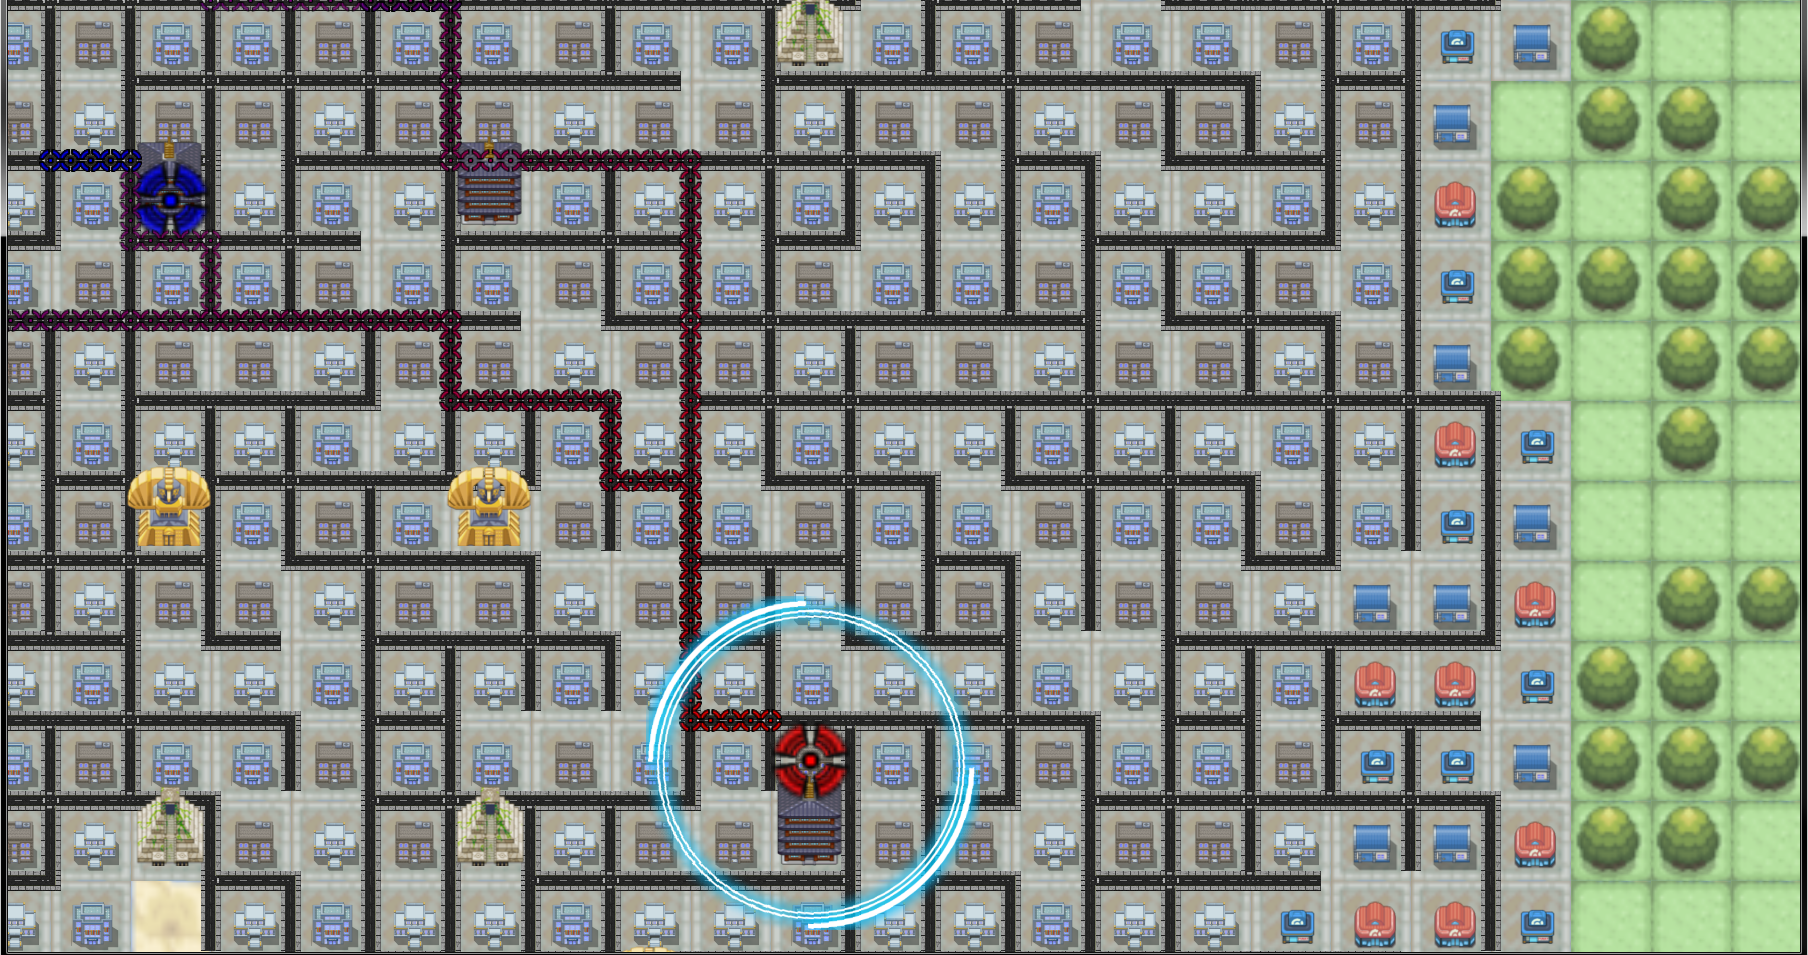
\includegraphics[scale=0.2]{img/exercise4}
\caption{Exercise 3.2 result}
\label{img:Ex3-2}
\end{figure}